\subsection{First approach}
\begin{frame}
\frametitle{First approach}

\begin{columns}
	\column{0.25\textwidth}
	\centering 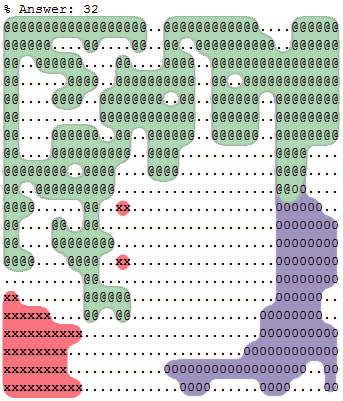
\includegraphics[width=0.7\textwidth]{images/adam.png}
	
	\column{0.75\textwidth}
	\begin{itemize}
		\item<1-> \textit{Answer Set Programming for Procedural Content Generation: A Design Space Approach} \textcolor{UDCpink}{[Smith et al, 11]}
		\item<2-> This approximation creates a single solid island.
		\item<3-> But we need more that one island.
	\end{itemize} 
\end{columns}
	
\end{frame}

\begin{frame}
\frametitle{First approach}

\begin{itemize}
	\item<1-> We created a starting point to generate an island.
	\item<2-> The program expanded these points with adjacency rules.
	\item<3-> We added the constrains rules so the adjacent islands wouldn't stick together.
	\item<4-> \textcolor{UDCpink}{Problem:} This approach was inefficient with large maps.
\end{itemize}

\end{frame}

\subsection{Second approach}

\begin{frame}
\frametitle{Second approach}

\begin{itemize}
	\item<1-> We divided the map in regions.
	\item<2-> One region is a single island.
	\item<3-> We used Lua built-in module clingo to call only one region generation.
	\item<4-> Once this worked, we generated all the regions with build-in module.
	\item<5-> Finally we added the restriction rules to the regions not stick together.
\end{itemize}

\end{frame}

\subsection{Related work}

\begin{frame}
\frametitle{Related work}

\begin{itemize}
	\item<1-> Add user restrictions to the generation.
	\item<2-> Add all types of terrain.
	\item<3-> Generate player starting points.
	\item<4-> Add a exporter to Freeciv map.
\end{itemize}

\end{frame}